\documentclass{math201}
\usepackage{hyperref}
\usepackage{bookmark}
\usepackage{minted}

% =============================================
% Part 0 信息
% =============================================

\mathsetup{
  % 学生姓名
  student = {某同学},
  % 学号
  student-id = {2021xxxx},
  % 院系
  experiment = {实验六 电容触摸屏实验},
  % 专业年级
  discipline = {集成电路设计与集成系统},
  % 日期
  date = {2024 年 4 月 9 日},
}

\begin{document}

% =============================================
% Part 1  封面
% =============================================

\makecover

% =============================================
% Part 2 主文档
% =============================================

\section{实验要求}

\begin{enumerate}
  \item 运行例程实验10 电容触摸屏-触摸画板实验 ,观察实验现象
  \item 看懂源程序
  \item 在LCD液晶屏上画一个红色框,一个蓝色框(具体坐标和大小自己定),修改源程序,实现:当触摸到红色框时显示I am red; 当触摸到蓝色框时显示I am blue; 当触摸其他位置时显示I am white;
\end{enumerate}

\section{实验内容及结果}

\subsection{编写代码}

需要修改 \texttt{gt9xx.c} 文件。

% \inputminted[
%     frame=lines,
%     framesep=2mm,
%     baselinestretch=1.2,
%     fontsize=\small,
%     linenos
% ]{C++}{code/gt9xx.c}

具体来说,需要修改的部分如下:

删除 \texttt{GTP\_Touch\_Down} 函数中的多余部分

\begin{minted}[
    frame=lines,
    framesep=2mm,
    baselinestretch=1.2,
    fontsize=\small,
]{C++}
static void GTP_Touch_Down(int32_t id,int32_t x,int32_t y,int32_t w)
{
  
  GTP_DEBUG_FUNC();

  /*取x、y初始值大于屏幕像素值*/
  GTP_DEBUG("ID:%d, X:%d, Y:%d, W:%d", id, x, y, w);

  /* 处理触摸按钮,用于触摸画板 */
  Touch_Button_Down(x,y); 
}
\end{minted}

仿照例程中的 \texttt{touch/palette.c} 和 \texttt{touch/palette.h},按要求编写以下代码。

\begin{enumerate}
  \item \texttt{show\_color.c} 功能:
  \begin{enumerate}
    \item 该代码用于在触摸屏上绘制颜色按钮。
    \item 按钮可以显示不同颜色的文本。
  \end{enumerate}
  \item \texttt{show\_color.h} 详细设计和实现要点:
  \begin{enumerate}
    \item 使用了 \texttt{NT35510} 驱动来控制液晶屏。
    \item 初始化了按钮的参数,包括位置、文本、颜色等。
    \item 通过触摸屏的回调函数 \texttt{Touch\_Button\_Down} 来处理按钮按下事件。
  \end{enumerate}
  \item \texttt{show\_color.h} 代码的注释:
  \begin{enumerate}
    \item \texttt{Delay} 函数是一个简单的延时函数。
    \item \texttt{Show\_Color\_Init} 函数用于初始化颜色显示。
    \item \texttt{Touch\_Button\_Init} 函数初始化按钮参数。
    \item \texttt{Touch\_Button\_Down} 函数处理按钮按下事件。
  \end{enumerate}
\end{enumerate}

总之,这段代码实现了在触摸屏上显示颜色按钮的功能。

\inputminted[
    frame=lines,
    framesep=2mm,
    baselinestretch=1.2,
    fontsize=\small,
    linenos
]{C++}{code/show_color.c}

\begin{enumerate}
  \item \texttt{show\_color.h} 功能:
  \begin{enumerate}
    \item 该代码用于在液晶屏上绘制颜色按钮。
    \item 按钮可以显示不同颜色的文本。
  \end{enumerate}

  \item \texttt{show\_color.h} 详细设计和实现要点:
  \begin{enumerate}
    \item 使用了 \texttt{NT35510} 驱动来控制液晶屏。
    \item 定义了一个名为 \texttt{Touch\_Button} 的结构体,用于存储按钮的参数,包括位置、文本、颜色等。
    \item 初始化了按钮的参数,例如按钮的起始坐标、结束坐标、文本内容和颜色。
    \item 实现了按钮按下事件的处理函数 \texttt{Touch\_Button\_Down}。
  \end{enumerate}

  \item \texttt{show\_color.h} 代码的注释:
  \begin{enumerate}
    \item \texttt{BUTTON\_WIDTH} 和 \texttt{BUTTON\_HEIGHT} 定义了按钮的宽度和高度。
    \item \texttt{BUTTON\_NUM} 定义了按钮的数量。
    \item \texttt{Touch\_Button} 结构体中的字段分别表示按钮的位置、颜色、文本等信息。
    \item \texttt{Show\_Color\_Init} 函数用于初始化颜色显示。
    \item \texttt{Touch\_Button\_Init} 函数初始化按钮参数。
  \end{enumerate}
\end{enumerate}

总之,这段代码实现了在液晶屏上显示颜色按钮的功能。

\inputminted[
    frame=lines,
    framesep=2mm,
    baselinestretch=1.2,
    fontsize=\small,
    linenos
]{C++}{code/show_color.h}

\subsection{下载运行}

使用 \texttt{FlyMCU.exe} 下载程序到 STM32 开发版上,观察实验现象。

\subsection{实验现象}

\begin{figure}[H]
  \centering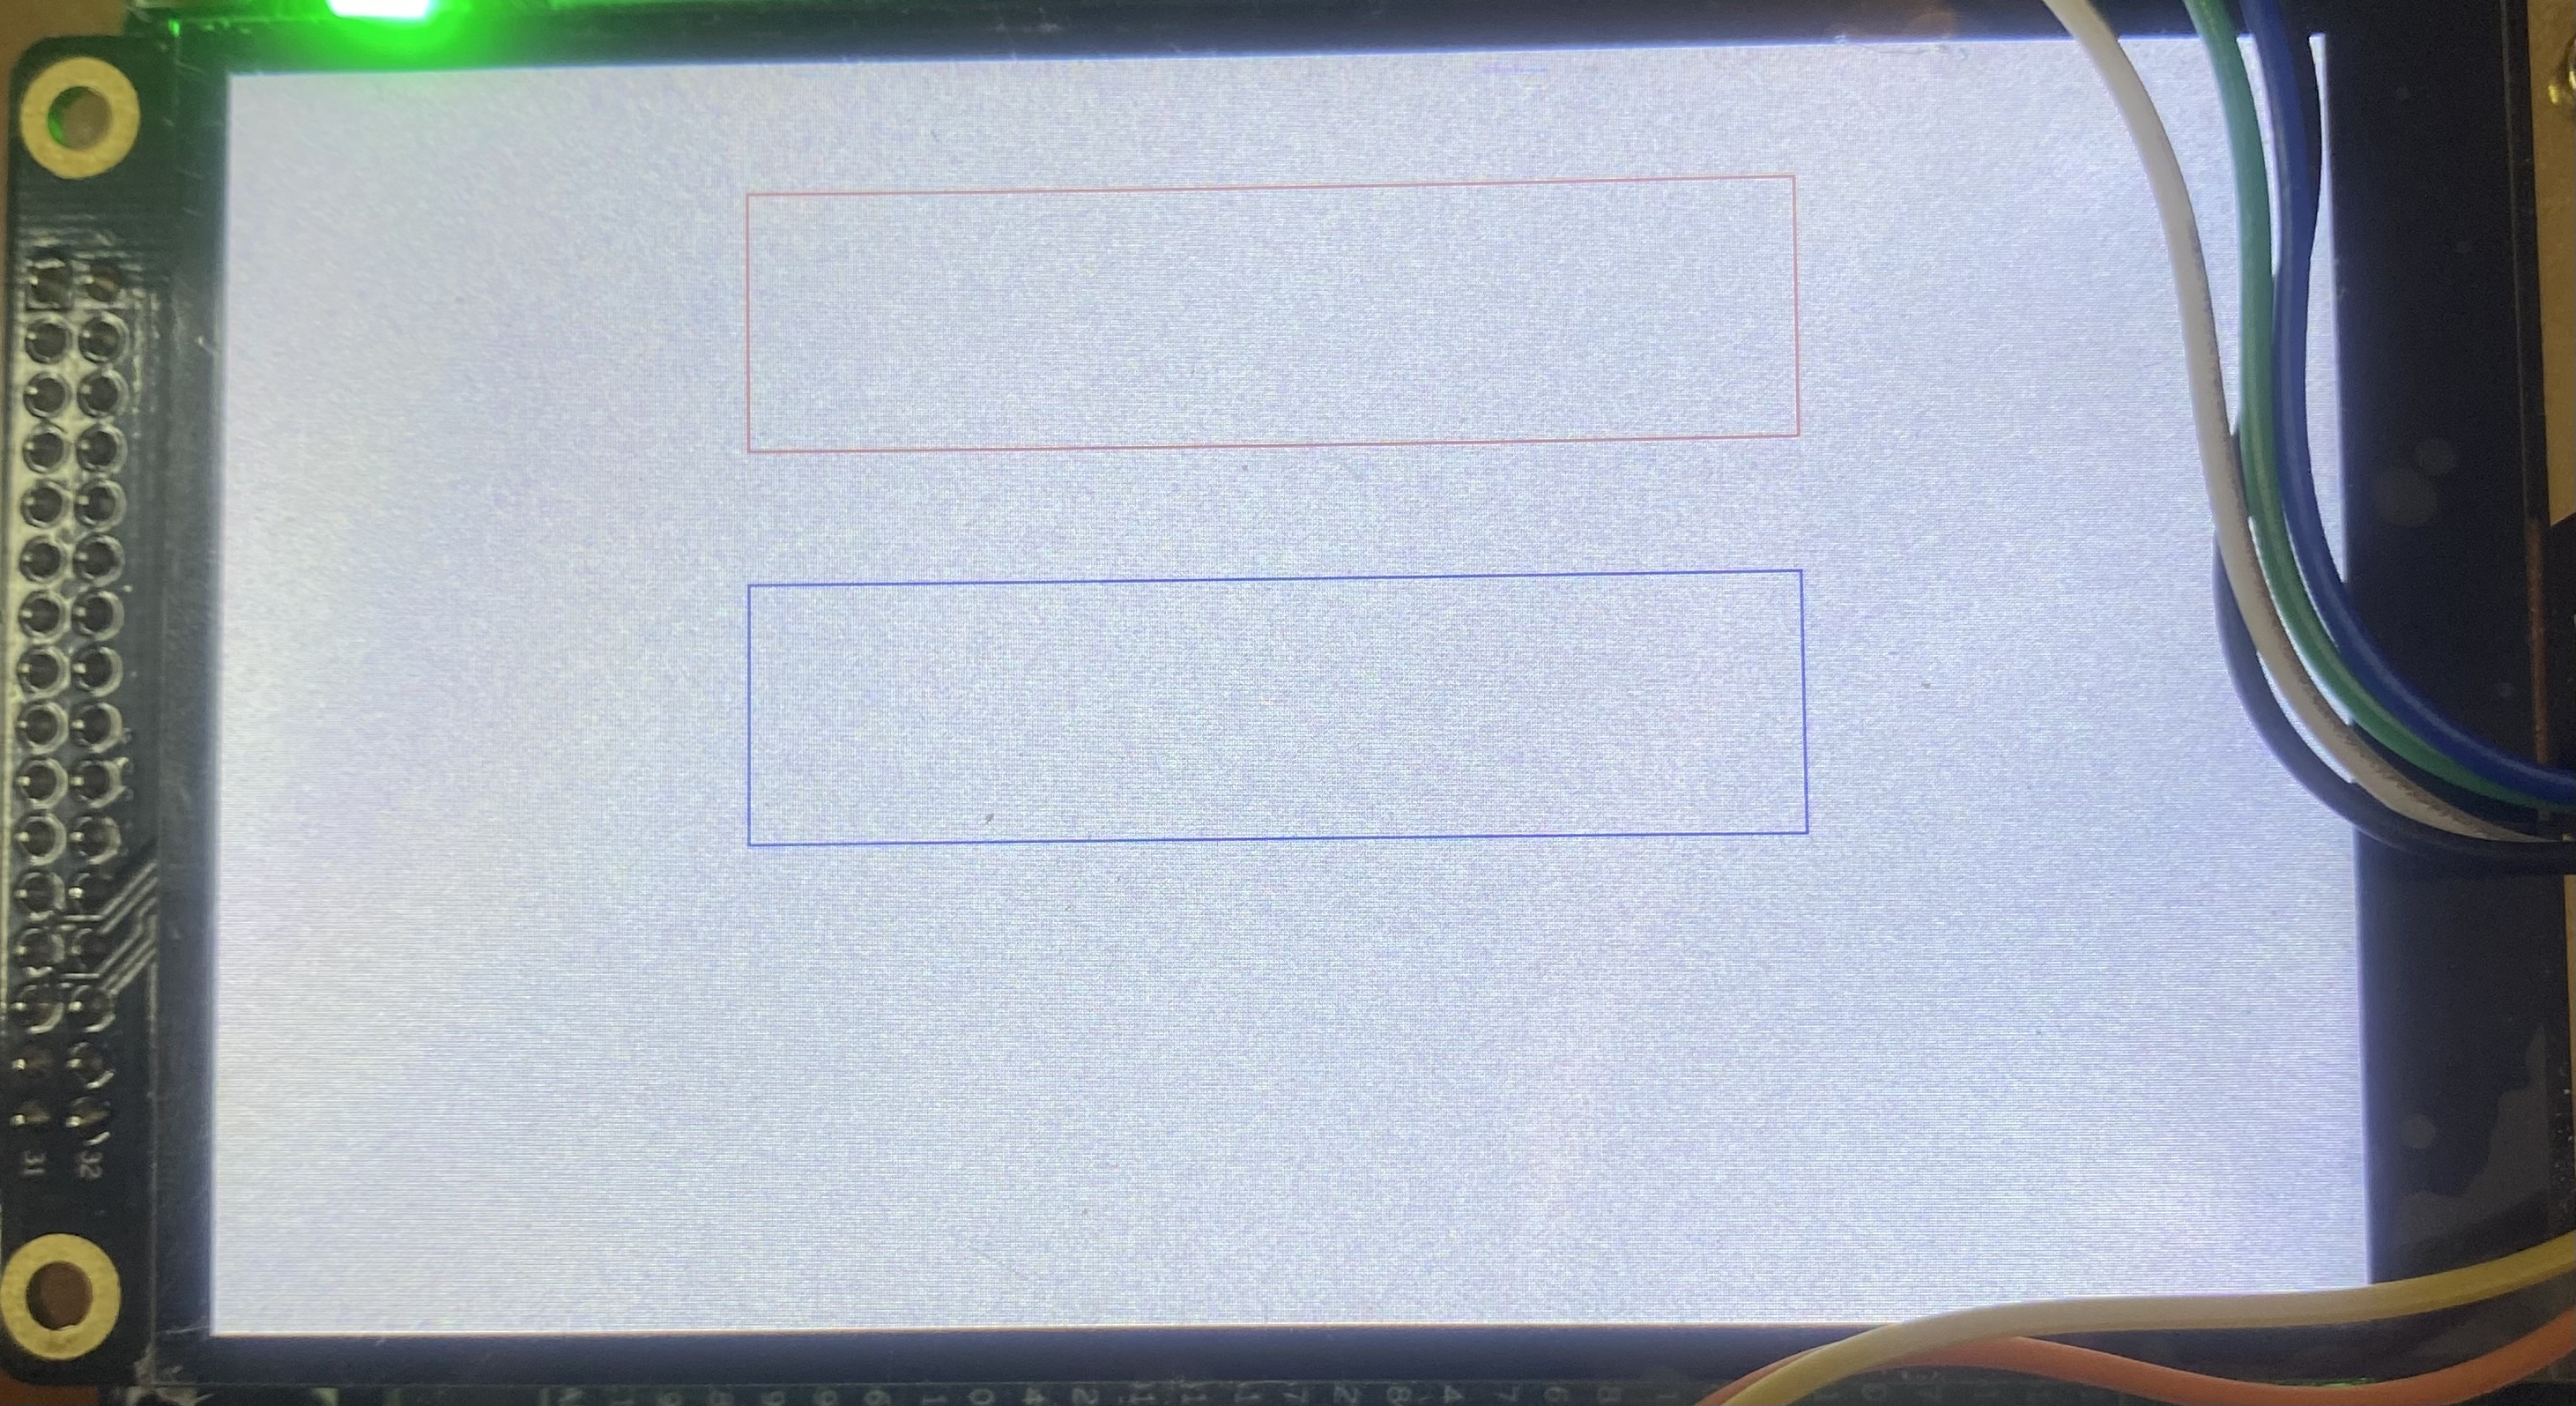
\includegraphics[width=0.6\linewidth]{touch_default.jpg}
  \caption{触摸屏默认显示}
\end{figure}

\begin{figure}[H]
   \centering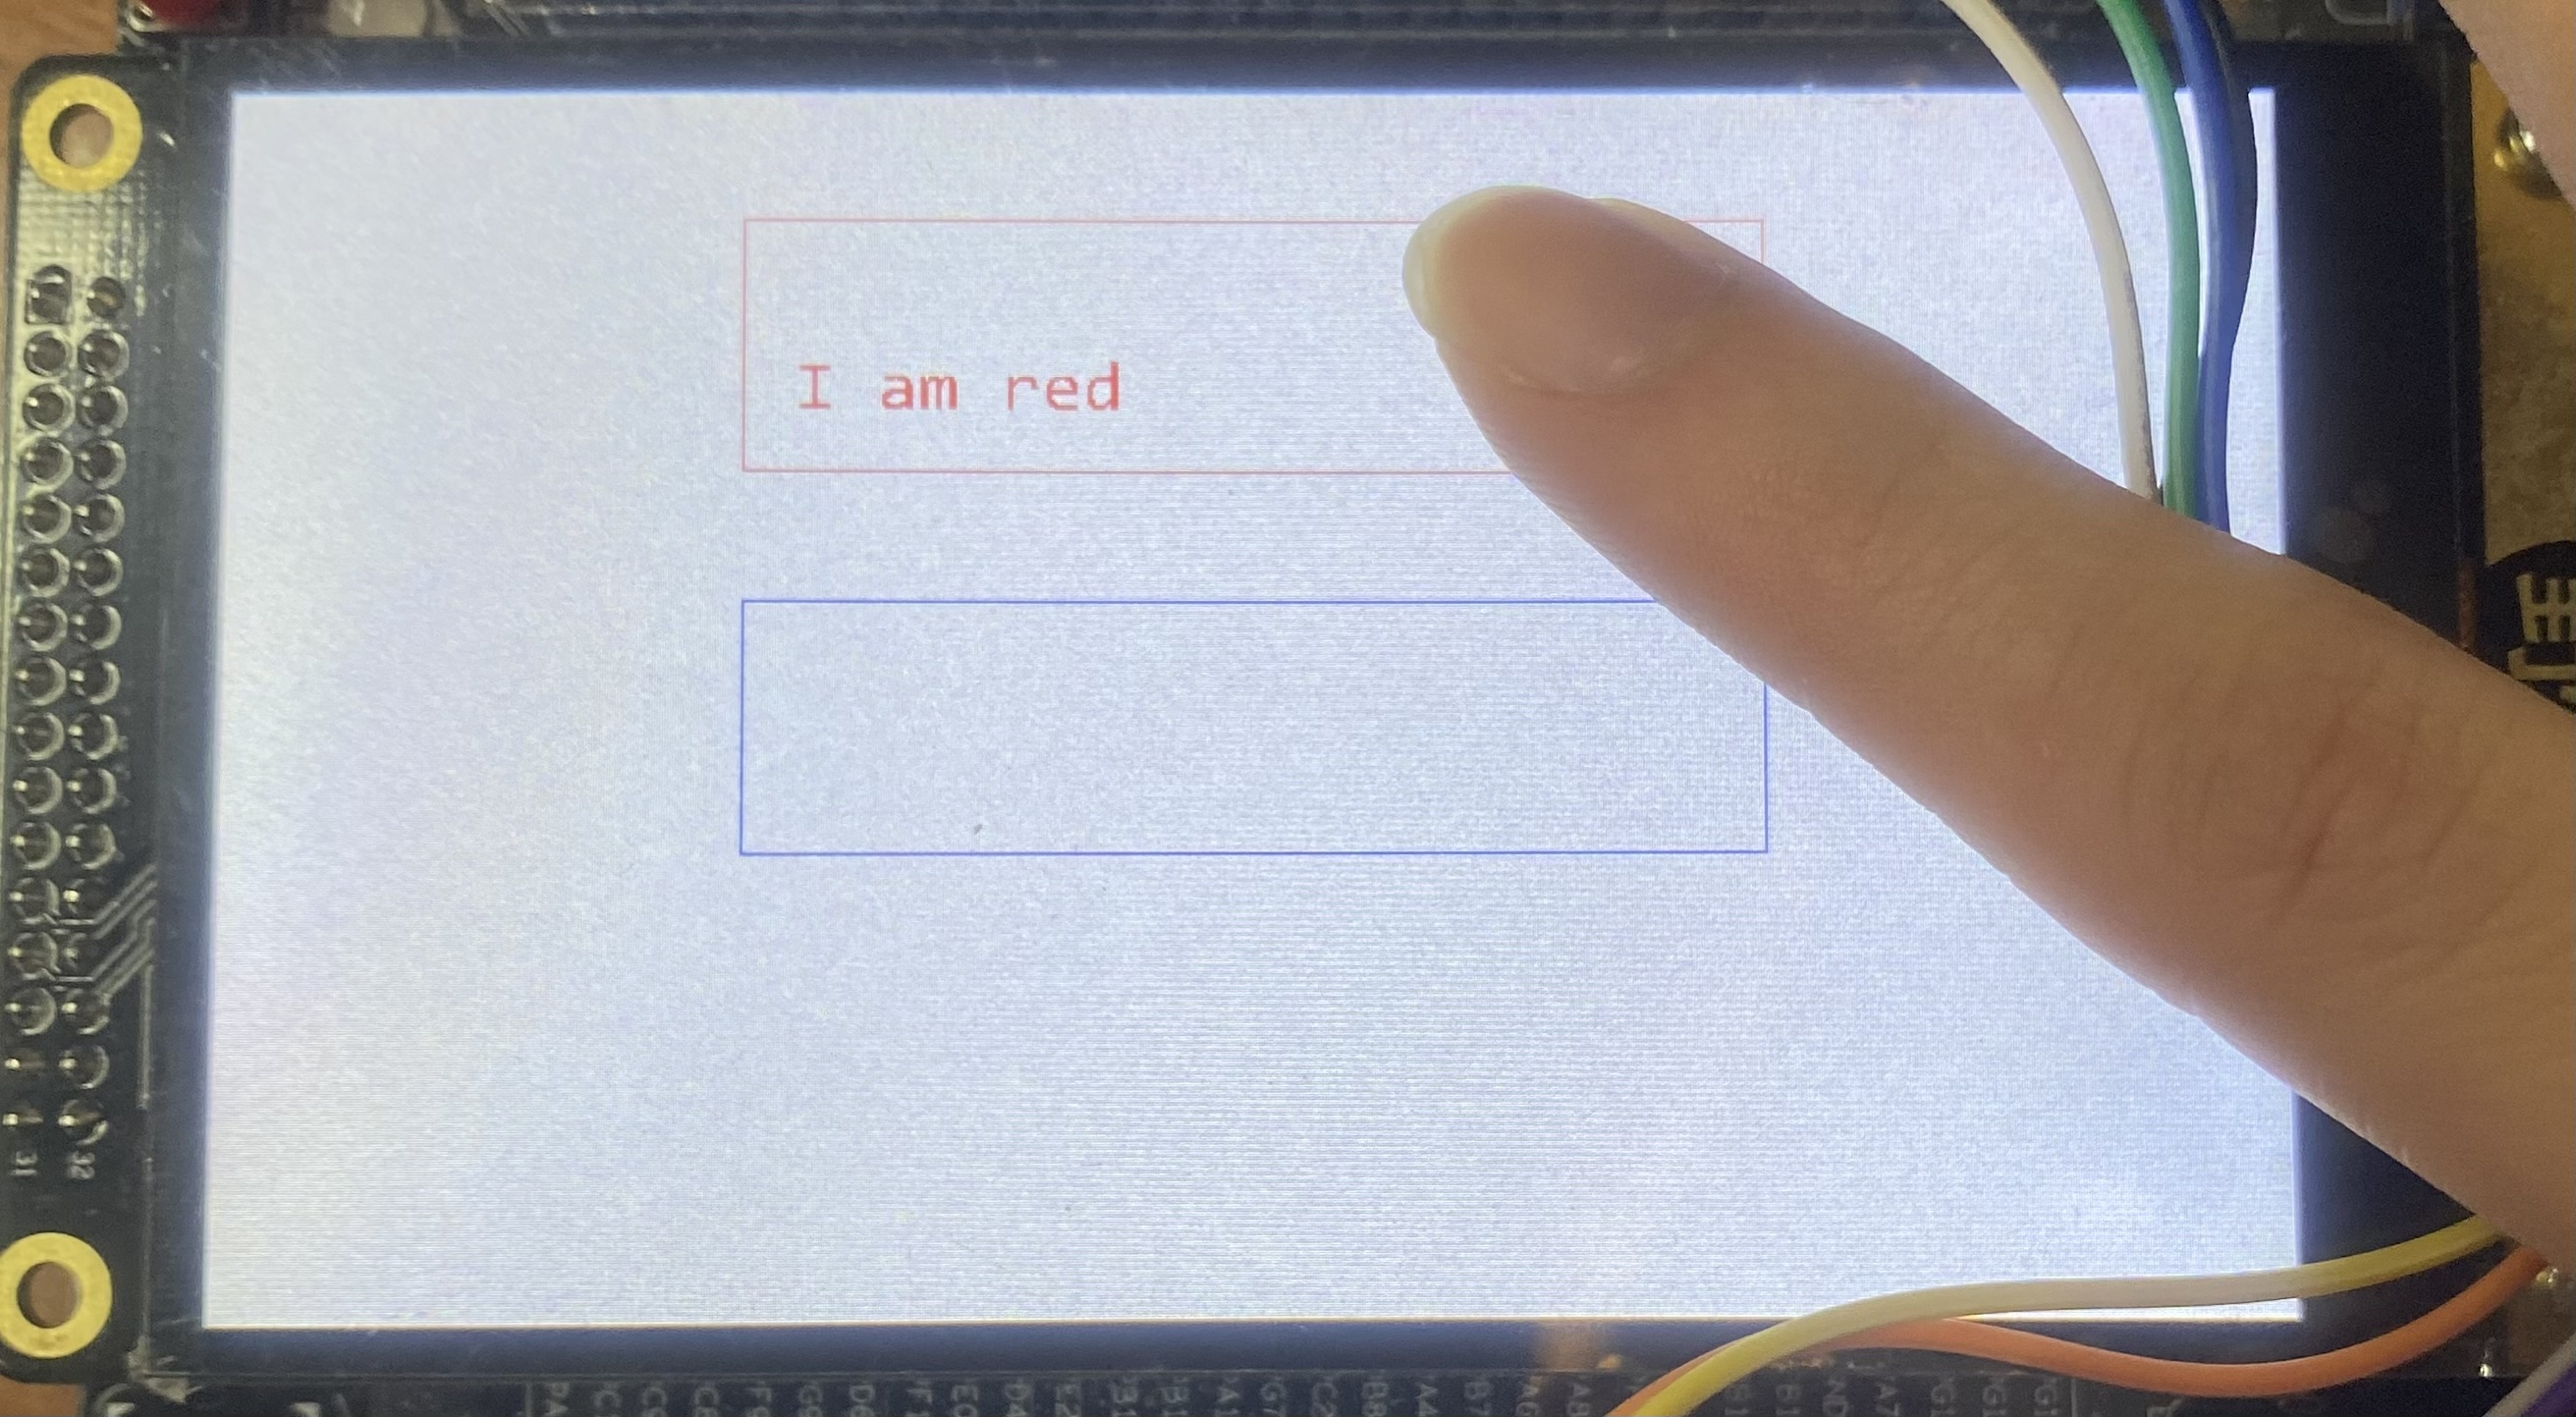
\includegraphics[width=0.6\linewidth]{touch_red.jpg}
   \caption{触摸屏红色显示}
\end{figure}

\begin{figure}[H]
   \centering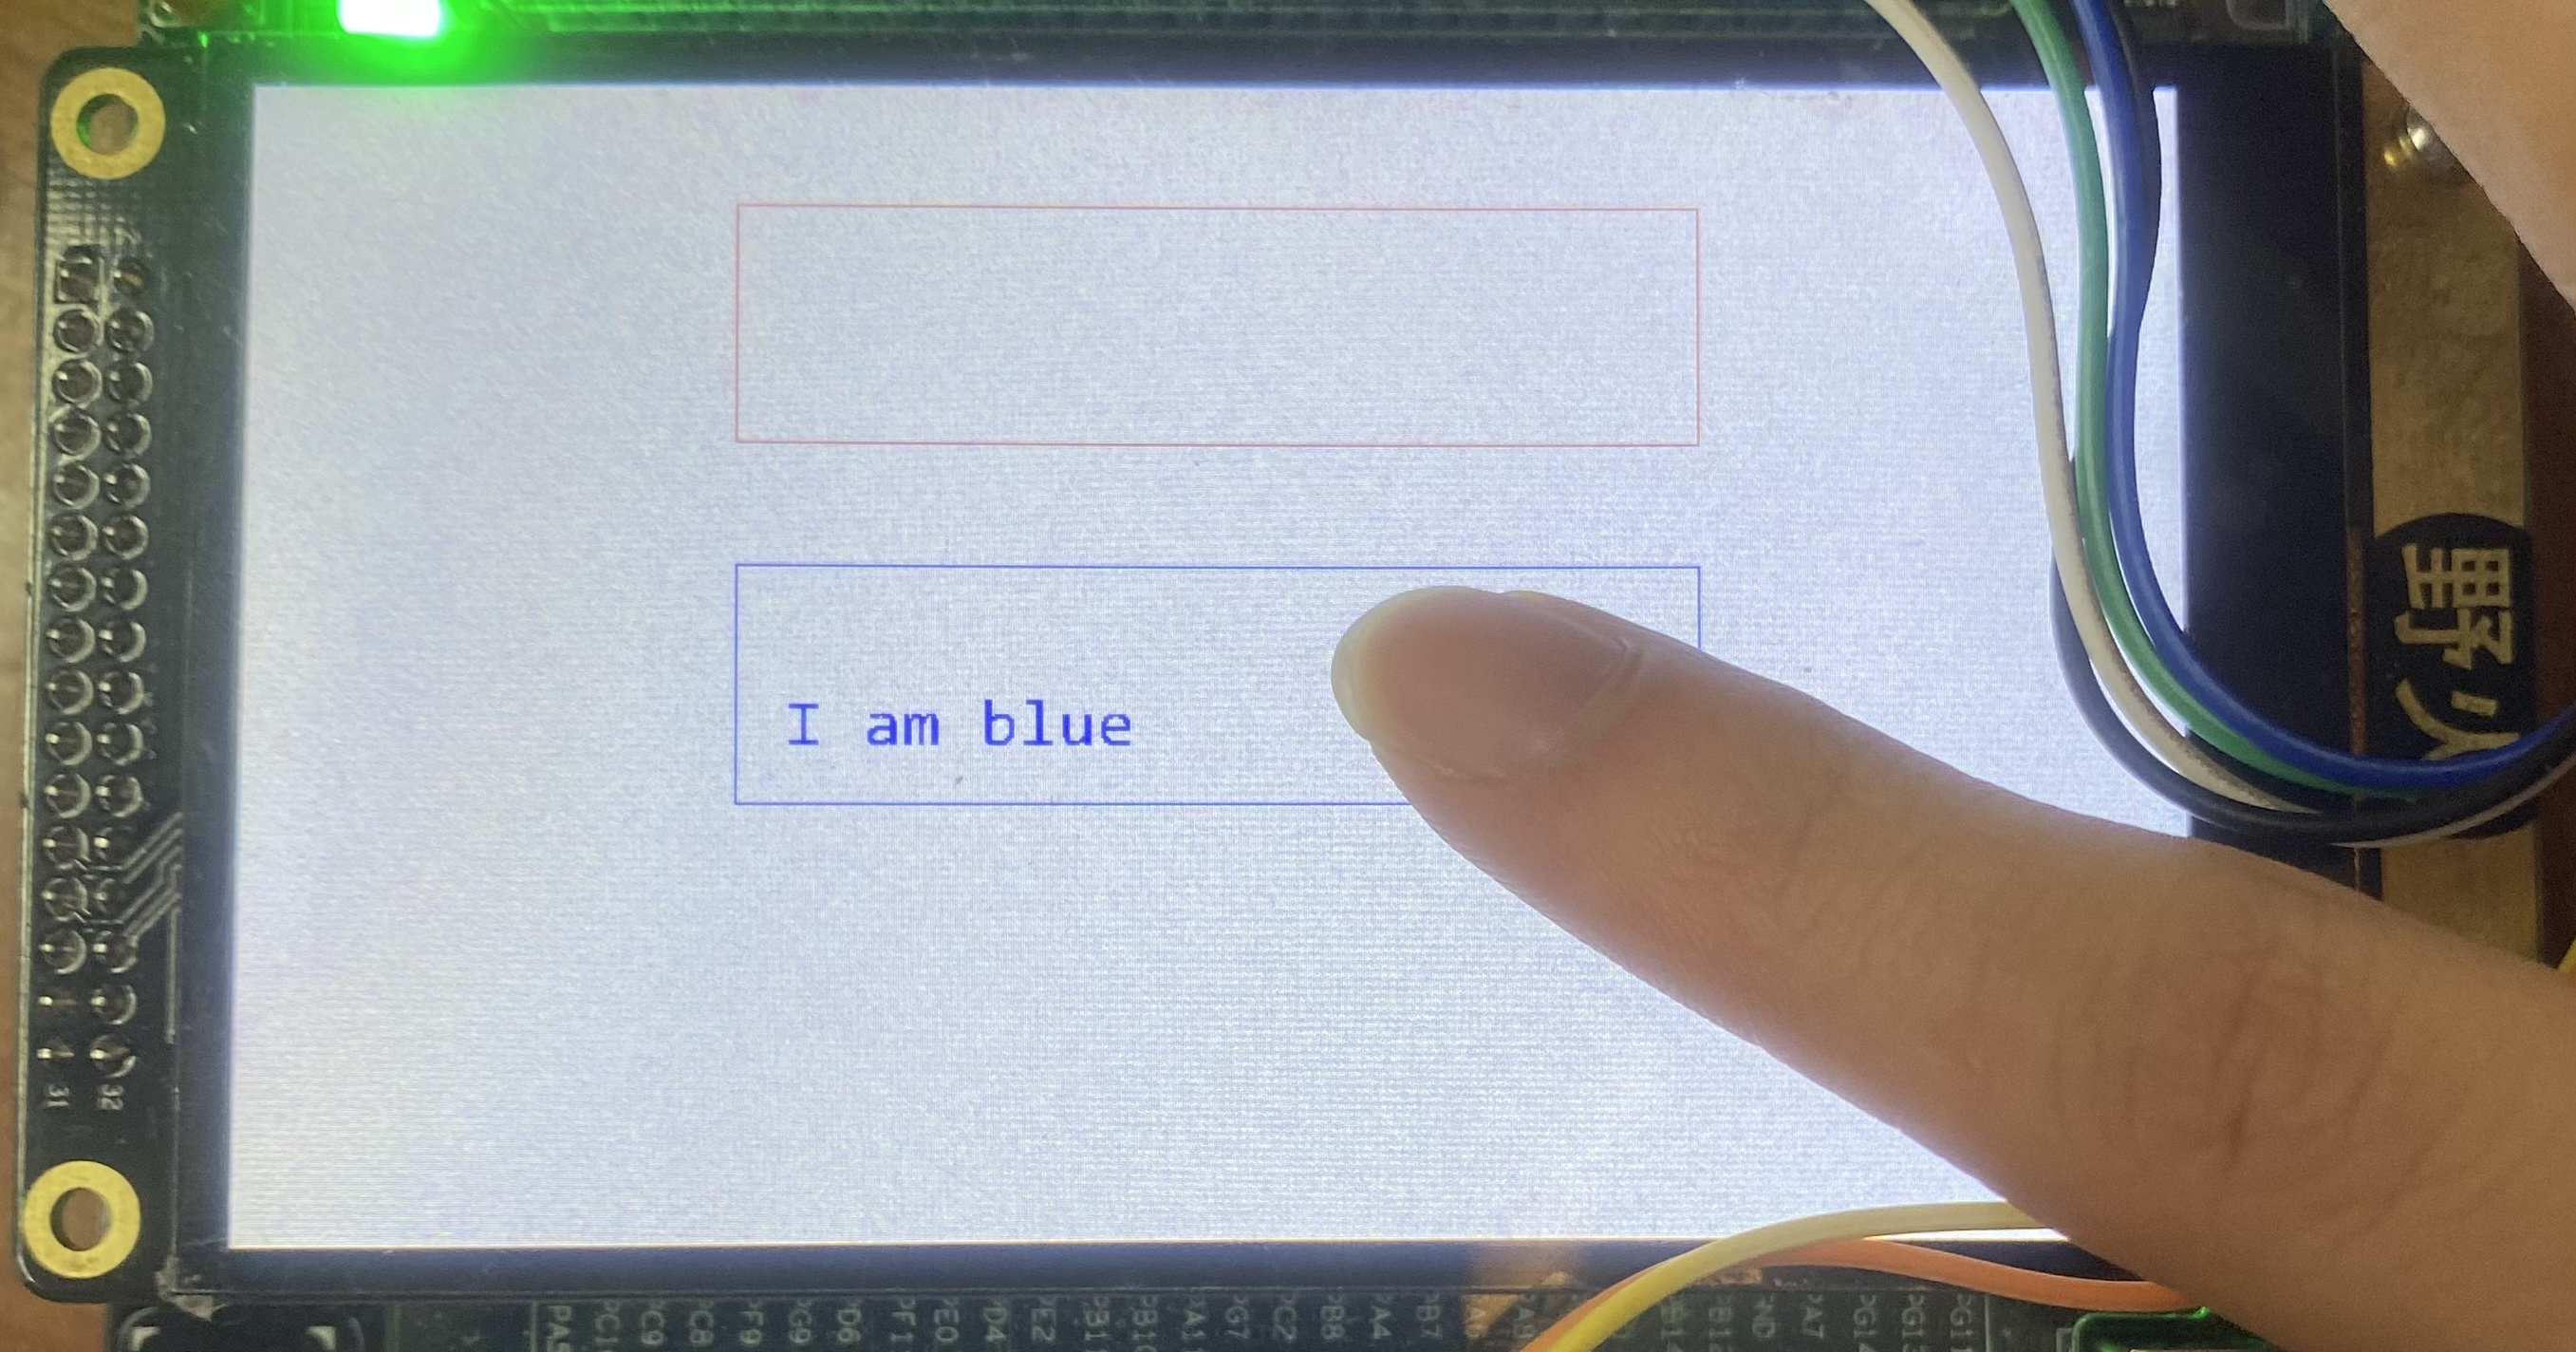
\includegraphics[width=0.6\linewidth]{touch_blue.jpg}
   \caption{触摸屏蓝色显示}
\end{figure}

\begin{figure}[H]
   \centering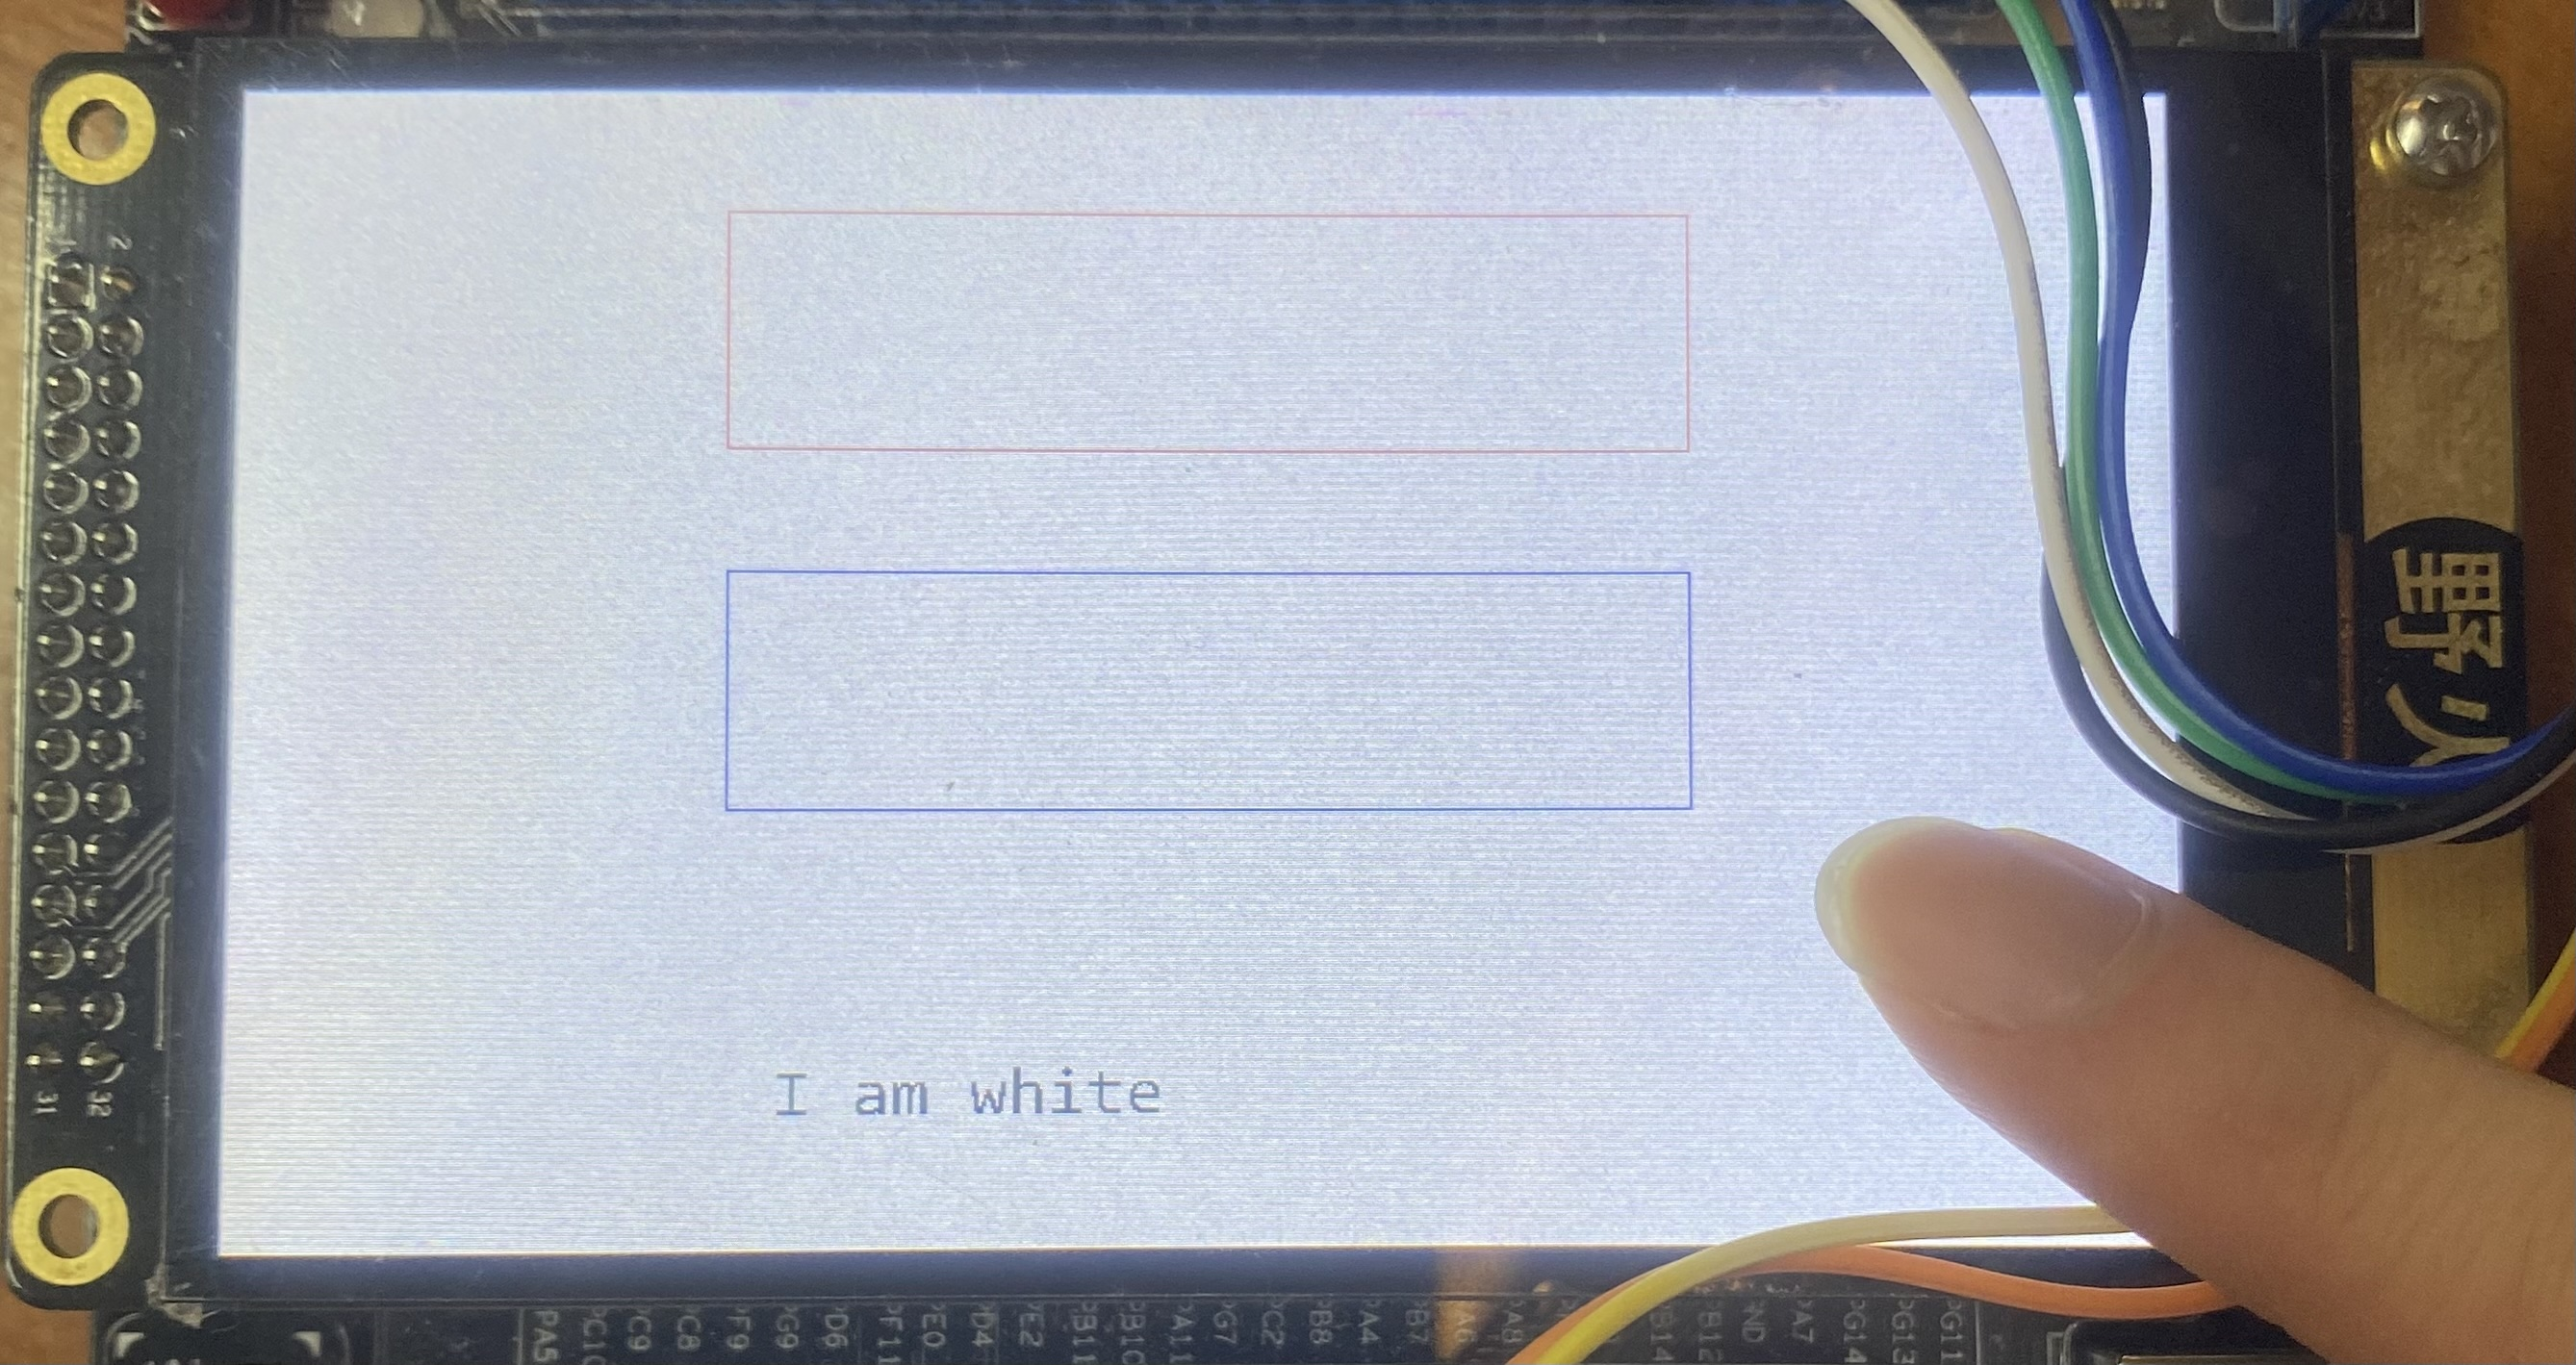
\includegraphics[width=0.6\linewidth]{touch_white.jpg}
   \caption{触摸屏白色显示}
 \end{figure}

\section{实验小结}

本次实验主要是通过修改源程序,实现了在触摸屏上显示不同颜色按钮的功能。通过触摸按钮,可以在液晶屏上显示不同的颜色文本。实验中,我学习了如何使用触摸屏的回调函数来处理按钮按下事件,以及如何在液晶屏上绘制颜色按钮。通过本次实验,我对触摸屏的使用有了更深入的了解,也提高了自己的编程能力。

\end{document}
